\documentclass[]{beamer}
% \geometry{papersize={16cm,9.60cm}}
\usepackage{etex}
\usepackage{amsmath}
\usepackage{tikz}
\usepackage{multimedia}
\usetheme{Boadilla}
\usepackage{graphicx}
%\usepackage{inputenc}

% \mode<presentation>
% {
%   \usetheme{default}
%   \setbeamercovered{transparent}
% }


% {\vskip5pt}

%% customize layout, bullet points navigation toolbar
\setbeamertemplate{navigation symbols}{}%remove navigation symbols
\setbeamertemplate{enumerate items}[default]
\setbeamertemplate{navigation symbols}{}
\setbeamertemplate{itemize items}[circle]
\setbeamercolor{enumerate item}{fg=black}

\setbeamertemplate{footline}{}
\setbeamersize{text margin left = 2.0em}
\setbeamersize{text margin right = 2.0em}

\usepackage{times}
\usepackage[T1]{fontenc}

% Or whatever. Note that the encoding and the font should match. If T1
% does not look nice, try deleting the line with the fontenc.

\setbeamertemplate{navigation symbols}{}

\title{ Cognitive (Neuro) Psychology }
\subtitle{VI. Scaling Methods}
\author{ Marianne Maertens }
\institute[TU Berlin]{Technische Universit\"at Berlin}
\date{July 2016}

\begin{document}
\setbeamertemplate{enumerate items}[default]
\setbeamertemplate{headline}

\frame{\titlepage}

\AtBeginSection[]
{
  \begin{frame}<beamer>
    \frametitle{Layout}
    \tableofcontents[currentsection]
  \end{frame}
}

\begin{frame}
 \frametitle{So far ...}
\begin{center}
\includegraphics<1>[width=100mm]{figs/l4/methods_overview_performance.png} 
\includegraphics<2>[width=100mm]{figs/l4/methods_overview_appearance.png} 
\end{center}
\end{frame}


\begin{frame}
 \frametitle{Perceptual Scales}
\begin{overlayarea}{110mm}{70mm}
describe the relationship between the \textcolor{blue}{perceived} and \textcolor{blue}{physical} magnitudes of a stimulus, e.g. transparency and perceived transparency

\begin{columns}[T]
 \begin{column}{50mm}
 \begin{itemize}
  \item[] ``psychological scales''
  \item[] ``sensory scales''
  \item[] ``transducer functions''
 \end{itemize}
 \end{column}

 \begin{column}{60mm}
\begin{center}
\includegraphics<2>[width=60mm]{figs/l6/perceived_transparency.png}
\includegraphics<1>[width=40mm]{figs/l6/knoblauch_scaling98.png}
\end{center}
 \end{column}
\end{columns}
\end{overlayarea}
\end{frame}


\begin{frame}
\frametitle{Matching vs. Scaling}
\begin{overlayarea}{110mm}{70mm}

\begin{columns}[T]
 \begin{column}{55mm}
\centering Adjust the test field so that it looks like the target
  \begin{center}
\includegraphics<1->[width=50mm]{figs/l6/ruler_matching.png}
 \end{center}
 \end{column}

 \begin{column}{55mm}
\only<2->{\centering Which of the pairs looks more different}
  \begin{center}
\includegraphics<2->[width=50mm]{figs/l6/ruler_mlds.png}
 \end{center}
 \end{column}
\end{columns}
\end{overlayarea}
\end{frame}



\begin{frame}
\frametitle{(Asymmetric) Matching}
\begin{overlayarea}{110mm}{60mm}
  \begin{center}
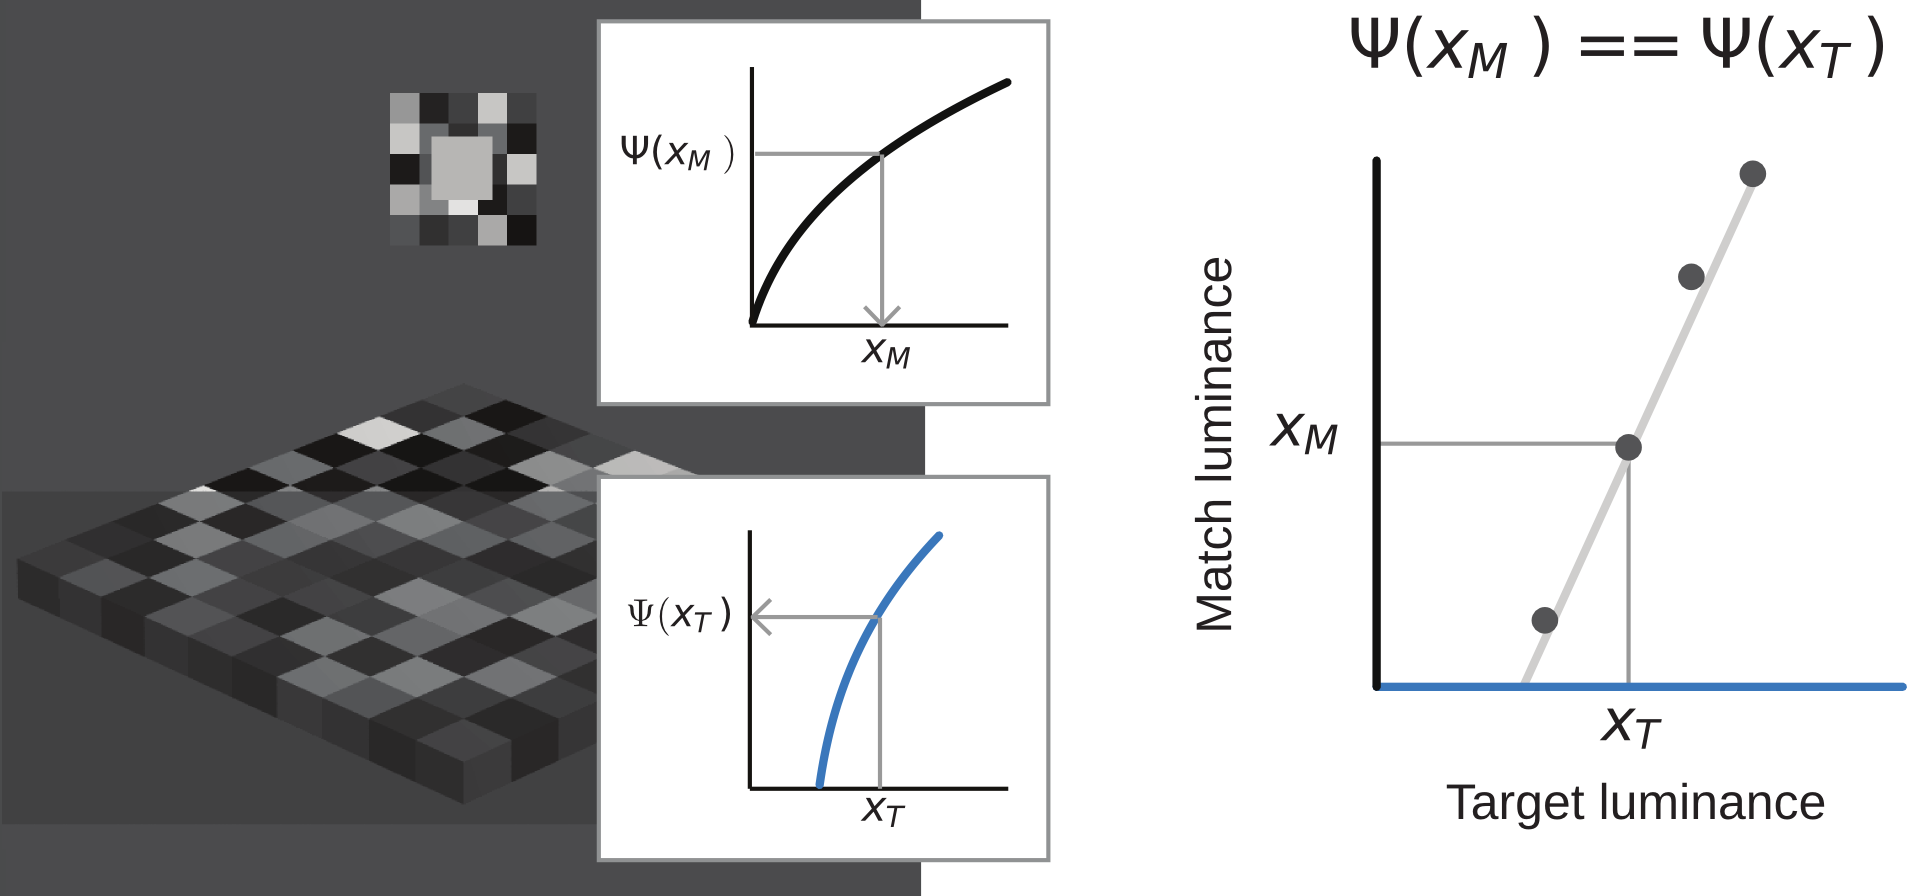
\includegraphics[width=110mm]{figs/l6/internal_functions_matching.png}
 \end{center}
\end{overlayarea}
\begin{itemize}
 \item<2-> matching measures internal variables indirectly
 \item<2-> it is prone to response strategies (Runeson!)
\end{itemize}
\end{frame}


\begin{frame}
 \frametitle{Types of perceptual scales}
\begin{overlayarea}{110mm}{60mm}
\begin{center}
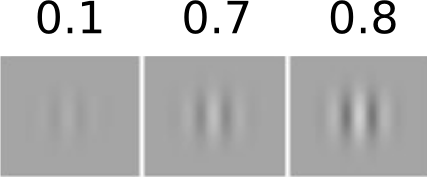
\includegraphics[width=50mm]{figs/l6/three_contrasts.png} 
\end{center}

\textcolor{blue}{ordinal:}
\begin{itemize}
 \item  number stimulus magnitudes according to their rank order along perceptual continuum, difference between any pair of number does not necessarily correspond to magnitude of the perceptual difference, e.g. 1, 2, 3 
 \item differences between numbers do not correspond to perceived differences
\end{itemize}
\end{overlayarea}
\end{frame}


\begin{frame}
 \frametitle{Types of perceptual scales}
\begin{overlayarea}{110mm}{60mm}
\begin{center}
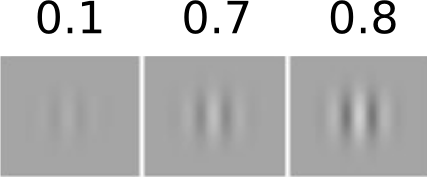
\includegraphics[width=50mm]{figs/l6/three_contrasts.png} 
\end{center}

\textcolor{blue}{interval:}
\begin{itemize}
 \item differences between number correspond to perceptual differences, even though numbers themselves are arbitrary, e.g. 1, 5, 6 or 4, 12, 14, an interval scale can be transformed without loss of information by the equation $aX+b$
 \item does not capture perceived relative magnitudes of the stimulus dimension
\end{itemize}
\end{overlayarea}
\end{frame}


\begin{frame}
 \frametitle{Types of perceptual scales}
\begin{overlayarea}{110mm}{60mm}
\begin{center}
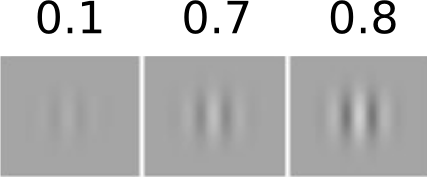
\includegraphics[width=50mm]{figs/l6/three_contrasts.png} 
\end{center}

\textcolor{blue}{ratio:}
\begin{itemize}
 \item capture relative perceived magnitudes, e.g. values of 1 and 5 indicate that the second value is five times the first 
\end{itemize}
\end{overlayarea}
\end{frame}


\begin{frame}
 \frametitle{Forced-choice vs. non-forced choice scaling procedures}
\begin{center}
\includegraphics<1>[width=90mm]{figs/l6/appearance_fc.png} 
\includegraphics<2>[width=90mm]{figs/l6/appearance_nonfc.png} 
\end{center}
\end{frame}

\begin{frame}
 \frametitle{Example: Multi-partition scaling}
\begin{center}
\includegraphics<1>[width=70mm]{figs/l6/whittle_display.png} 
\includegraphics<2>[width=70mm]{figs/l6/whittle_scale.png} 
\end{center}
\end{frame}



\begin{frame}
 \frametitle{General principle of a perceptual scale}
 
\begin{itemize}
 \item perceptual scale is power function $\Psi(x) = a*S^n$
 \item quadruples
 \item equal physical magnitudes, different perceptual magnitudes and vice versa
\end{itemize}

\begin{center}
\includegraphics<1>[width=90mm]{figs/l6/scale_power_function.pdf} 
\end{center}
\end{frame}


\begin{frame}
 \frametitle{Perceptual scales and internal noise}
\begin{overlayarea}{110mm}{70mm}
Why not construct a perceptual scale from JNDs?\\

\only<2->{
\vspace{5mm}
\textcolor{blue}{thought experiment:}
\begin{itemize}
 \item start with low stimulus level, baseline
 \item measure JND between baseline and a higher stimulus level
 \item second baseline will be first baseline plus the JND
 \item measure JND between second baseline and a higher stimulus
 \item ...
 \item series of baselines separated by JNDs that span the entire stimulus range
 \item[=] Discrimination scale, Discrimination or Fechnerian scaling 
\end{itemize}
}
\end{overlayarea}
\end{frame}


\begin{frame}
 \frametitle{Perceptual scales and internal noise}
\begin{overlayarea}{110mm}{90mm}
\begin{itemize}
 \item JND for some criterion level, e.g. 75\% correct, depends on signal-to-noise ratio $\frac{\Delta\Psi}{\sigma}$
\end{itemize}

\begin{center}
  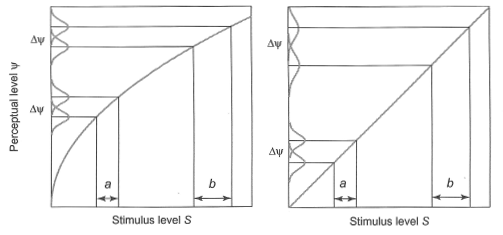
\includegraphics[width=90mm]{figs/l6/additive_noise.png}
\end{center}

\begin{columns}[T]
 \begin{column}{35mm}
\begin{itemize}
 \item \textit{additive}  noise
\end{itemize}
   \end{column}
 \begin{column}{40mm}
 \begin{itemize}
 \item \textit{multiplicative} noise 
 \end{itemize}
 \end{column}
\end{columns}
\begin{itemize}
 \item<2->[$\Rightarrow$] impossible to derive the shape of the underlying perceptual scale from JNDs
\end{itemize}
\end{overlayarea}
\end{frame}



\begin{frame}
 \frametitle{Maximum Likelihood Difference Scaling - MLDS \\ \scriptsize{Maloney \& Yang, 2003}}
 
\normalsize
\begin{itemize}
 \item forced-choice scaling procedure
 \item state-of-the-art optimization
 \item produces interval perceptual scale
\end{itemize}
\end{frame}



\begin{frame}
 \frametitle{How MLDS works}
\begin{itemize}
 \item set of stimulus magnitudes $S_1, S_2, S_3, ..., S_n$
 \item $\Psi(2), \Psi(3), \Psi(4), ..., \Psi(n-1)$ are free parameters that have to be estimated, $\Psi(1)$ and $\Psi(n)$ are fixed at 0 and 1
 \item[]
 \item<2-> trial 1: $S_1,S_2$ and $S_3,S_4$, 
 \item<2-> observer: $S_1,S_2$ is more different 
 \item<2-> for a given test set of $\Psi(S)$s MLDS calculates the probability that a hypothetical observer characterized by these parameters will respond that $S_1,S_2$ has the larger perceived difference = likelihood for this trial
 \item[] 
 \item<3-> likelihoods of all trials are multiplied to obtain across-trials likelihood
\end{itemize}
\end{frame}


\begin{frame}
 \frametitle{Single trial example}
\begin{overlayarea}{120mm}{80mm}
\begin{itemize}
 \item initial guesses for parameters:
 \item[] $\Psi(1)=0.5$, $\Psi(2)=0.7$, $\Psi(3)=0.2$, $\Psi(4)=0.3$ 
 \item internal decision noise is: $\sigma_d=0.1$
 \item[]
 \item[$\Rightarrow$] $L(S_1,S_2)|(\Psi(1),\Psi(2),\Psi(3),\Psi(4))$
 \item[]
\end{itemize}
\only<2->{
 $D = |\Psi(2)-\Psi(1)| - |\Psi(4)-\Psi(3)| = |(0.7-0.5)|-|0.3-0.2| = 0.1$
}
\begin{itemize}
\item[] 
\item<3-> convert to z-score $\frac{D}{\sigma_d} = 1$
 \item<3-> calculate area under the standard normal distribution $\Phi(z=1)=0.8413$
 \item[]
 \item<4->[$\Rightarrow$] $L(S_3,S_4)|(\Psi(1),\Psi(2),\Psi(3),\Psi(4)) = (1-0.8413)$
\end{itemize}
\end{overlayarea}
\end{frame}


\begin{frame}
 \frametitle{Across-trials likelihood}
\begin{overlayarea}{120mm}{80mm}
\begin{enumerate}
\setlength{\itemsep}{10pt}
 \item calculate likelihoods for all trials
 \item multiply individual likelihoods across trials
 \item compute logarithm of the result
 \item repeat procedure for other set of $\Phi(S)$ and $\sigma_d$
 \item select the set that gives the largest across-trials likelihood
\end{enumerate}
\end{overlayarea}
\end{frame}



\begin{frame}
\frametitle{MLDS at work - constructing a lightness scale}

\begin{overlayarea}{130mm}{60mm}
\begin{center}
 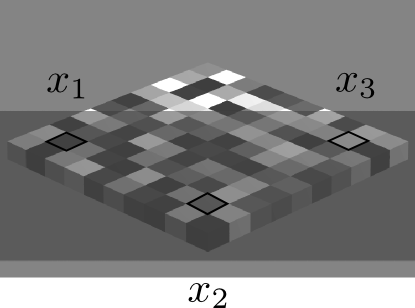
\includegraphics[width=60mm]{figs/l6/adelson_triad.png}

\vspace{5mm}
\only<1>{
\textit{``Which pair looks more different, $(x_1, x_2)$ or $(x_2,x_3)$?"}}
\end{center}

\only<2->{
\begin{itemize}
 \item[] \textbf{Decision model:} $\Delta = (\Psi(x_3)-\Psi(x_2))-(\Psi(x_2)-\Psi(x_1)) + \epsilon$, 
 \item[] \hspace{30mm} $\epsilon \sim N(0,\sigma^2)$
\end{itemize}}
\end{overlayarea}
\end{frame}



\begin{frame}
\frametitle{MLDS at work - constructing a lightness scale}
\begin{center}
 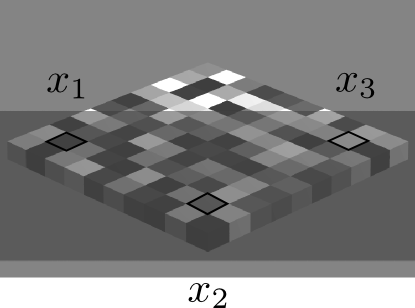
\includegraphics[width=40mm]{figs/l6/adelson_triad.png}
\vspace{3mm}

 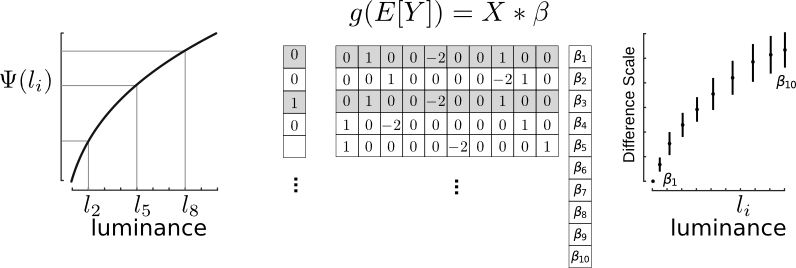
\includegraphics[width=100mm]{figs/l6/mlds_model.png}
\end{center}
\end{frame}

\begin{frame}
\frametitle{MLDS at work - constructing a lightness scale}
\begin{overlayarea}{110mm}{60mm}
\begin{columns}[T]
\begin{column}{50mm}
\begin{center}
 \includegraphics<1->[width=50mm]{figs/l6/mlds_scale_contrast.png}
\end{center}
 \end{column}

\begin{column}{50mm}
\begin{itemize}
 \item human observers are more sensitive to differences in low intensities
\end{itemize}

\end{column}
\end{columns}
\end{overlayarea}
\end{frame}

\begin{frame}
\frametitle{Relevance: electronic displays}
\begin{overlayarea}{110mm}{80mm}
\textbf{Gamma correction} is the name of a nonlinear operation used to encode luminance values in image systems. Gamma correction is defined by the following power-law expression:
\begin{itemize}
\item[] $V_{out} = V_{in}^{\gamma}$
\item[] Mac 2.1, Windows 2.2
\end{itemize}

\begin{columns}[T]
\begin{column}{50mm}
\begin{center}
 \includegraphics<1->[width=50mm]{figs/l6/mlds_scale_contrast.png}
\end{center}
 \end{column}

\begin{column}{50mm}
\begin{center}
 \includegraphics<1->[width=50mm]{figs/l6/gamma_functions.png}
\end{center}
\end{column}
\end{columns}
\end{overlayarea}
\end{frame}


\begin{frame}
 \frametitle{ Applications}
\begin{overlayarea}{110mm}{70mm}
\begin{columns}[T]
 \begin{column}{60mm}
  \begin{itemize}
  \setlength{\itemsep}{5pt}
   \item<1-> Standardized color palettes e.g. Munsell
   \item<1-> Monitor calibration
   \item<2-> Colormaps in plotting software
  \end{itemize}
 \end{column}

 \begin{column}{50mm}
  \includegraphics<1->[width=30mm]{figs/l6/munsell_color_wheel.png}
 \end{column}
\end{columns}

\begin{center}
 \includegraphics<2->[width=100mm]{figs/l6/matplotlib_option_a.png}
\end{center}
\end{overlayarea}
\end{frame}


\begin{frame}
 \frametitle{Summary}
\begin{itemize}
 \item forced-choice scaling: paired, triad, quadruple comparison
 \item non-forced-choice scaling: partition, multi-partition scaling
 \item[]  
 \item discrimination (Fechnerian) scaling is appropriate when the scale is used to \textit{predict} JNDs 
 \item to use a JND based scale to identify the true underlying perceptual scale, internal noise must be additive
 \item[]
 \item MLDS is relevant for a variety of applications
\end{itemize}
\end{frame}


\begin{frame}
 \frametitle{References}
\begin{small}
\begin{itemize}
 \item  Kingdom, F.A.A. \& Prins, N. (2010). Psychophysics. A practical introduction. London, UK: Elsevier Academic Press.
\end{itemize}
\end{small}
\end{frame}

\end{document}